\documentclass[10pt,a4paper]{article}
\usepackage[T1]{fontenc}
\usepackage[utf8]{inputenc}
\DeclareUnicodeCharacter{2212}{\ensuremath{-}}
\DeclareUnicodeCharacter{2192}{\ensuremath{\rightarrow}}
\DeclareUnicodeCharacter{2014}{---}
\usepackage{lmodern,amsmath,amssymb,graphicx,booktabs,tabularx,array}
\usepackage[margin=18mm,headheight=14pt]{geometry}
\usepackage{xcolor,tikz,tcolorbox,listings,enumitem,fancyhdr,lastpage}
\usetikzlibrary{arrows.meta,positioning}
\usepackage[unicode,colorlinks=true,linkcolor=blue!45!black,urlcolor=blue!45!black]{hyperref}
\definecolor{navy}{HTML}{173650}
\definecolor{accent}{HTML}{1766A7}
\definecolor{pale}{HTML}{EDF4FA}
\definecolor{amber}{HTML}{8A550B}
\setlength{\parindent}{0pt}\setlength{\parskip}{5pt}
\renewcommand{\arraystretch}{1.18}
\setlist[enumerate]{leftmargin=*,itemsep=3pt,topsep=3pt}
\setlist[itemize]{leftmargin=*,itemsep=2pt,topsep=3pt}
\hyphenpenalty=1500\emergencystretch=2em\raggedbottom
\pagestyle{fancy}\fancyhf{}
\fancyhead[L]{\small\textcolor{navy}{MyModelRobot | pierwsze ruchy i programy}}
\fancyhead[R]{\small Instrukcja laboratoryjna}
\fancyfoot[L]{\scriptsize Wersja robocza: 14.11.2026}
\fancyfoot[R]{\small\thepage\,/\,\pageref{LastPage}}
\newcommand{\ui}[1]{\textbf{\textsf{#1}}}
\newcommand{\cmd}[1]{\texttt{#1}}
\newcommand{\page}[2]{\clearpage{\Large\bfseries\color{navy}#1}\par{\small\color{accent}#2}\par\vspace{3pt}}
\newtcolorbox{goal}{colback=pale,colframe=accent,boxrule=.5pt,arc=2mm,left=2mm,right=2mm,top=1mm,bottom=1mm}
\newtcolorbox{remember}{colback=yellow!6,colframe=amber,boxrule=.5pt,arc=2mm,left=2mm,right=2mm,top=1mm,bottom=1mm}
\lstset{basicstyle=\ttfamily\small,columns=fullflexible,keepspaces=true,breaklines=true,frame=single,rulecolor=\color{blue!20},backgroundcolor=\color{pale},xleftmargin=2mm,xrightmargin=2mm,aboveskip=5pt,belowskip=5pt,showstringspaces=false}
\hypersetup{pdftitle={MyModelRobot - cwiczenia wprowadzajace},pdfsubject={Uczenie punktow, uklady wspolrzednych i programowanie ruchu},pdfauthor={Material pomocniczy do zajec robotyki}}
\begin{document}
{\Huge\bfseries\color{navy} MyModelRobot}\par
{\LARGE Pierwsze ruchy i programy robota}\par
\textcolor{accent}{Samodzielny zestaw ćwiczeń wprowadzających}\par
\begin{goal}
Po zajęciach potrafisz poruszać robotem w trybach Joint, World i Tool, nauczyć dwa punkty, zaplanować i odtworzyć ruch, rozpoznać ograniczenie kinematyczne lub kolizję oraz zapisać kompletny projekt.
\end{goal}
\textbf{Organizacja.} Ćwiczenia 1--6: około 90 minut; ćwiczenie 7 i rozszerzenia: dodatkowe 20--30 minut. Pracuj w parze: jedna osoba steruje, druga zapisuje obserwacje. Nie jest wymagana znajomość innych symulatorów ani języków programowania robotów.

\textbf{Uruchomienie.} Otwórz \cmd{standalone.html} z dostarczonego katalogu aplikacji albo adres podany przez prowadzącego. Wybierz język \ui{EN}, aby nazwy przycisków odpowiadały instrukcji. Pliki i obliczenia pozostają w przeglądarce; połączenie z robotem fizycznym nie jest potrzebne.

\begin{enumerate}
\item Wybierz \ui{Start programming}, a na małym ekranie zakładkę \ui{Program}.
\item Rozwiń \ui{Start here} i naciśnij \ui{Teach two poses}. Zostaną zastąpione bieżąca scena i program; własną pracę wcześniej zapisz do ZIP.
\item Sprawdź: robot \cmd{classroom\_six\_axis\_arm}, świat \cmd{two\_pose\_lesson}, TCP \cmd{tcp\_link}. Robot powinien być zgięty, a komunikat o kierunkach kartezjańskich dodatni.
\item Na dużym ekranie panel nauczania może być odłączony. Przeciągnij jego belkę tak, aby widzieć robota, lub użyj \ui{Dock}. Widok można obracać myszą; \ui{Fit robot} dopasowuje kamerę.
\end{enumerate}

\begin{center}
\begin{tikzpicture}[n/.style={draw=accent,fill=pale,rounded corners,align=center,font=\small,minimum height=11mm,text width=29mm},>=Stealth]
\node[n](a){Wczytaj\linebreak stanowisko};\node[n,right=4mm of a](b){Poruszaj\linebreak i ucz punkty};\node[n,right=4mm of b](c){Przywróć\linebreak początek};\node[n,right=4mm of c](d){Plan path\linebreak potem Play};\node[n,right=4mm of d](e){Zapisz ZIP\linebreak i sprawdź};
\foreach \x/\y in {a/b,b/c,c/d,d/e}\draw[->,thick,accent](\x)--(\y);
\end{tikzpicture}
\end{center}

\begin{tabularx}{\linewidth}{@{}lX@{}}\toprule
\textbf{Gdzie pracujesz?}&\textbf{Do czego służy?}\\\midrule
\ui{Program}&Panel nauczania, źródło programu, planowanie, odtwarzanie i komunikaty.\\
\ui{Workcell}&Przykłady całych stanowisk, otwieranie i zapis projektu ZIP, scena SDF.\\
\ui{Files / URDF}&Osobne wczytanie opisu robota i siatek oraz edycja jego modelu.\\
\ui{Joints / Animation}&Dodatkowe narzędzia pracy ze złączami i animacją CSV; w tym zestawie używaj przede wszystkim panelu nauczania.\\\bottomrule
\end{tabularx}
\begin{remember}\textbf{Najważniejsze jednostki:} pozycja w metrach, kąty w radianach. \(1\,\mathrm{cm}=0.01\,\mathrm{m}\), \(10^\circ\approx0.1745\,\mathrm{rad}\). Symulator opisuje ruch kinematyczny; nie wyznacza sił kontaktu ani nie realizuje sterowania sprzętem.\end{remember}

\page{1. Poznaj robota i trzy tryby ruchu}{Około 15 min | stanowisko: Teach two poses}
\begin{goal}\textbf{Cel:} odróżnić ruch pojedynczego złącza od ruchu TCP w układzie świata i narzędzia. TCP to wybrany układ końcówki robota; jego początek jest punktem programowania.\end{goal}
\begin{center}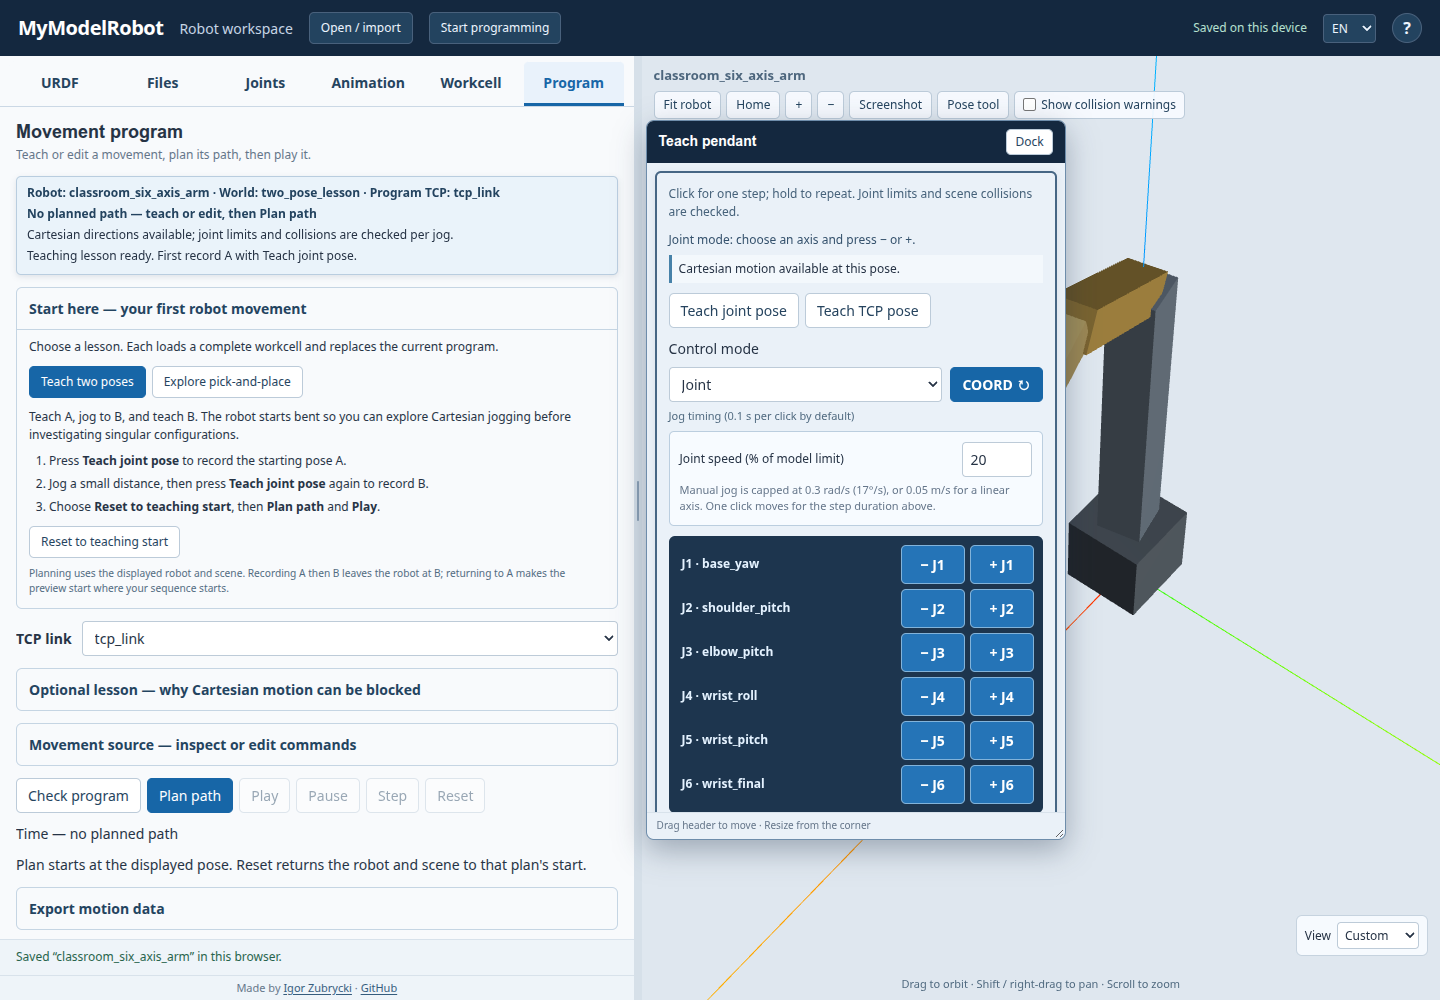
\includegraphics[width=.83\linewidth]{assets/start.png}\\[-1mm]{\footnotesize Widok orientacyjny. Nazwy i kolejność działań podano w tekście.}\end{center}
\vspace{-3mm}
\begin{enumerate}
\item W panelu \ui{Teach pendant} wybierz \ui{Joint}. Kliknij raz \ui{+J1}, a następnie \ui{−J1}. Powtórz dla J2 i J5. Obserwuj, które człony się poruszają. Przytrzymanie przycisku powtarza kroki.
\item Otwórz \ui{TCP and joint values / last velocity request}. Zapisz pozycję TCP i jedną współrzędną złączową. Jeden krok trwa domyślnie \(0.1\,\mathrm{s}\); ustawienie jest pod \ui{Jog timing}.
\item Użyj \ui{Reset to teaching start}. Wybierz \ui{World TCP} lub przycisk \ui{COORD}. Ustaw prędkość liniową \(0.01\,\mathrm{m/s}\). Kliknij \ui{+X}; odczytaj zmianę \(x,y,z\). Dla jednego kroku oczekuj zmiany około \(1\,\mathrm{mm}\), o ile ruch nie został spowolniony.
\item Ponownie przywróć początek. Wybierz \ui{Tool TCP} i kliknij \ui{+X}. Przy zgiętym, obróconym narzędziu zmieni się zwykle więcej niż jedna składowa pozycji w świecie.
\item W trybie Tool wypróbuj mały obrót \ui{+Rz}. To obrót wokół lokalnej osi narzędzia. W trybie World ta sama etykieta odnosi się do osi świata.
\end{enumerate}
\begin{tabularx}{\linewidth}{@{}lXXX@{}}\toprule
Tryb i próba&Co pozostaje zadane?&Zaobserwowane \(\Delta x,\Delta y,\Delta z\)&Wniosek\\\midrule
Joint, +J1&Jedno złącze&\rule{0pt}{8mm}&\\
World, +X&Kierunek świata&\rule{0pt}{8mm}&\\
Tool, +X&Kierunek narzędzia&\rule{0pt}{8mm}&\\\bottomrule
\end{tabularx}
\textbf{Zaliczenie:} poprawne wskazanie różnicy World/Tool i trzech poruszonych złączy. \textbf{Pytanie:} czy ruch +X w Tool musi zwiększać współrzędną \(x\) w świecie? Uzasadnij obserwacją.

\page{2. Naucz dwa punkty i uruchom swój program}{Około 15 min | świeże Teach two poses}
\begin{goal}\textbf{Cel:} zbudować i wykonać program A~\(\rightarrow\)~B oraz świadomie określić stan początkowy.\end{goal}
\begin{enumerate}
\item Wczytaj świeże \ui{Teach two poses}. Wybierz \ui{Teach joint pose}. Powstaje nazwany cel oraz polecenie \cmd{MOVEJ}.
\item W trybie Joint kliknij raz \ui{+J1}. Naciśnij \ui{Teach joint pose} ponownie. To drugi punkt.
\item Rozwiń \ui{Movement source}. Znajdź \cmd{ROBOT}, \cmd{TOOL}, dwa wiersze \cmd{JOINTS} i dwa wiersze \cmd{MOVEJ}. Nazwy wygenerowane przez aplikację mogą różnić się od A i B poniżej.
\item Naciśnij \ui{Reset to teaching start}, potem \ui{Plan path}. Sprawdź stan gotowości, niebieski podgląd toru i czas ruchu. Samo planowanie nie oznacza odtwarzania.
\item Naciśnij \ui{Play}. Sprawdź końcową wartość J1. Wypróbuj \ui{Pause}, \ui{Reset} i \ui{Step}.
\end{enumerate}
\textbf{Minimalny program do samodzielnego wpisania.} Poniższy wariant jest przeznaczony wyłącznie dla świeżej lekcji z robotem \cmd{classroom\_six\_axis\_arm}. Wklej go w pole źródła zamiast programu lekcji.
\begin{lstlisting}
ROBOT classroom_six_axis_arm
TOOL tcp_link
JOINTS A base_yaw=0.2 shoulder_pitch=-0.5 elbow_pitch=0.8 wrist_roll=0.3 wrist_pitch=-0.4 wrist_final=0.2
JOINTS B base_yaw=0.23 shoulder_pitch=-0.5 elbow_pitch=0.8 wrist_roll=0.3 wrist_pitch=-0.4 wrist_final=0.2
MOVEJ A
MOVEJ B
\end{lstlisting}
\textbf{Kopiowanie:} gotowy tekst jest w \cmd{examples/02\_two\_poses.robot}. Długie wiersze \cmd{JOINTS} mogą być zawinięte na wydruku, lecz każdy cel musi zajmować jeden logiczny wiersz w źródle aplikacji.
\begin{remember}\textbf{Punkt A nie staje się automatycznie początkiem planowania.} Plan powstaje z aktualnie wyświetlonej konfiguracji i sceny. Po nauczeniu B robot stoi w B. Bez jawnego powrotu do A zobaczysz najpierw ruch B~\(\rightarrow\)~A, a potem A~\(\rightarrow\)~B. \ui{Reset to teaching start} jest natychmiastowym przywróceniem lekcji, nie zaplanowanym ruchem.\end{remember}
\begin{center}\begin{tikzpicture}[>=Stealth,font=\small]
\node at (0,1){Nauka};\draw[->,thick,accent](1,1)--(7,1);\node[above] at(1,1){zapis A};\node[above] at(7,1){zapis B};
\node[anchor=east] at(0,0){Odtwarzanie};\draw[->,thick,accent](1,0)--(7,0);\node[below,anchor=north west]at(1,0){najpierw przywróć A};\node[below]at(7,0){osiągnięcie B};
\end{tikzpicture}\end{center}
\textbf{Uwaga o stanie:} edycja źródła unieważnia plan, ale zachowuje wyświetloną pozycję. \ui{Reset} przy gotowym planie przywraca jego robot, scenę i relacje z obiektami do stanu początkowego. \ui{Step} przechodzi do kolejnej próbki czasowej, nie do kolejnego polecenia języka.

\textbf{Zaliczenie:} dwa cele, odtworzony ruch i zapisane wartości J1 w A/B. \textbf{Pytanie:} dlaczego po zmianie programu trzeba ponownie użyć Plan path?

\page{3. Odcinek i łuk: zaprogramuj geometrię toru}{Około 15 min | Workcell → Load weld-path example}
\begin{goal}\textbf{Cel:} rozróżnić ruch do celu \cmd{MOVEJ}, odcinek TCP \cmd{MOVEL} i łuk TCP \cmd{MOVEC}. Użyj prostego robota kartezjańskiego; w tym ćwiczeniu pomijamy proces spawania.\end{goal}
Wczytaj \ui{Workcell → Load weld-path example}. W \ui{Program} zastąp źródło poniższym programem. Nazwy \cmd{a}, \cmd{v}, \cmd{b} są nazwami pozycji TCP. Orientacja \cmd{Q 0 0 0 1} oznacza brak obrotu względem wskazanego układu \cmd{world}.
\begin{lstlisting}
ROBOT seam_cartesian
TOOL tcp_link
POSE a world 0.15 0    0 Q 0 0 0 1
POSE v world 0.35 0.14 0 Q 0 0 0 1
POSE b world 0.55 0    0 Q 0 0 0 1
MOVEJ a
MOVEL v
MOVEL b
MOVEL a
PAUSE 0.5
MOVEC v b
MOVEL a
\end{lstlisting}
\begin{center}
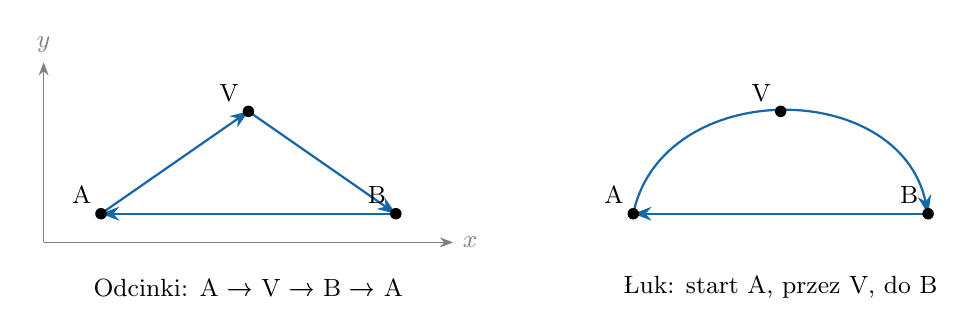
\begin{tikzpicture}[scale=1.04,>=Stealth,font=\small]
\draw[->,gray](0,0)--(5,0)node[right]{\(x\)};\draw[->,gray](0,0)--(0,2.2)node[above]{\(y\)};
\coordinate(a)at(.7,.35);\coordinate(v)at(2.5,1.6);\coordinate(b)at(4.3,.35);
\draw[thick,accent,->](a)--(v);\draw[thick,accent,->](v)--(b);\draw[thick,accent,->](b)--(a);
\foreach \n/\lab in {a/A,v/V,b/B}{\fill(\n)circle(2pt)node[above left]{\lab};}
\node at(2.5,-.55){Odcinki: A → V → B → A};
\begin{scope}[xshift=6.5cm]
\coordinate(a)at(.7,.35);\coordinate(v)at(2.5,1.6);\coordinate(b)at(4.3,.35);
\draw[thick,accent,->](a) .. controls(1.05,2.02)and(3.95,2.02)..(b);
\draw[thick,accent,->](b)--(a);
\foreach \n/\lab in {a/A,v/V,b/B}{\fill(\n)circle(2pt)node[above left]{\lab};}
\node at(2.5,-.55){Łuk: start A, przez V, do B};
\end{scope}
\end{tikzpicture}
\end{center}
\textit{Schemat ideowy, bez skali; dokładny okrąg wyznacza aplikacja z trzech punktów.}
\begin{enumerate}
\item Użyj \ui{Check program}, potem \ui{Plan path} i \ui{Play}. Przejdź na widok z góry, aby zobaczyć różnicę między wielokątem i łukiem.
\item Wskaż, skąd \cmd{MOVEC v b} bierze trzeci punkt. Jest nim bieżący start ruchu, tutaj A po ostatnim \cmd{MOVEL a}.
\item Po \ui{Reset} zmień wartość \(y\) punktu V o niewielką wartość, np. do \(0.10\). Zaplanuj ponownie i porównaj kształt. Jeśli tor jest niewykonalny, zachowaj komunikat i wróć do wariantu początkowego.
\end{enumerate}
\textbf{Zaliczenie:} zrzut podglądu obu fragmentów i wyjaśnienie roli punktu V. \textbf{Pytanie:} dlaczego \cmd{MOVEJ} do tego samego celu nie gwarantuje odcinka TCP?

\page{4. Rozpoznaj ograniczenie i odzyskaj sterowanie}{Około 10--15 min | świeże Teach two poses}
\begin{goal}\textbf{Cel:} rozróżnić ograniczenie geometrii, prędkości i kolizję; reagować na komunikat zamiast wielokrotnie naciskać ten sam przycisk.\end{goal}
\begin{enumerate}
\item Wczytaj świeżą lekcję. Rozwiń \ui{Optional lesson — why Cartesian motion can be blocked}. Użyj \ui{Set straight posture for this exercise}. To celowy, natychmiastowy reset demonstracyjny.
\item Odczytaj ostrzeżenie o ograniczeniu ruchu kartezjańskiego. W World naciśnij \ui{+X}. Przy wyprostowanym ramieniu ten kierunek, przy zachowaniu orientacji, powinien zostać zablokowany. Sprawdź, że współrzędne złączy się nie zmieniły.
\item Rozwiń szczegóły ostatniego żądania. Wskaż żądaną i uzyskaną prędkość oraz resztę błędu. To diagnostyka kinematyki prędkości; nie są to siły ani błąd pomiaru robota.
\item Wybierz \ui{Switch to Joint mode to recover}. Małym ruchem J2/J3 lub J5 zmień postawę. Pojedynczy obrót J1 nie musi usuwać utraty dostępnego kierunku. Najprostszy powrót do sprawdzonej konfiguracji: \ui{Reset to teaching start}.
\item W zgiętej postawie porównaj pojedynczy World +Z dla prędkości liniowej \(0.01\) i \(0.05\,\mathrm{m/s}\), przy tej samej długości kroku. Przed każdą próbą przywróć tę samą konfigurację. Zapisz zmianę pozycji i ewentualny współczynnik automatycznego spowolnienia.
\end{enumerate}
\begin{tabularx}{\linewidth}{@{}p{40mm}XX@{}}\toprule
\textbf{Co widzisz?}&\textbf{Znaczenie}&\textbf{Co zrobić?}\\\midrule
Near singular / restricted&Niektóre kierunki są trudne lub lokalnie niedostępne.&Zmienić postawę w Joint; ponowić mały krok.\\
Automatically slowed&Ograniczenia złączy wymagały mniejszej prędkości.&Odczytać zastosowany procent; nie oczekiwać pełnego przesunięcia nominalnego.\\
Position limit&Złącze osiągnęło granicę położenia.&Wybrać przeciwny kierunek; nie wyłączać ograniczeń.\\
Collision&Próbkowany ruch narusza geometrię kolizyjną.&Odczytać parę nazw, sprawdzić scenę/tor i przywrócić poprawny stan.\\
No planned path&Źródło lub stan zmieniły się; nie ma aktualnego planu.&Po zakończeniu zmian użyć Plan path.\\\bottomrule
\end{tabularx}
\begin{remember}Zmniejszenie prędkości nie tworzy brakującego kierunku ruchu. Automatyczne spowolnienie dotyczy wykonalnego kierunku ograniczonego prędkościami lub krokiem przy granicy złącza. Po nieudanym kroku aplikacja zachowuje stan robota.\end{remember}
\textbf{Zaliczenie:} opis zablokowanej próby i skutecznego powrotu do sterowania; tabela dwóch prędkości. \textbf{Pytanie:} czy siedem złączy gwarantuje możliwość dowolnego ruchu TCP w każdej konfiguracji?

\page{5. Przenieś obiekt: pierwszy cykl pick-and-place}{Około 15 min | Workcell → Load pick-and-place example}
\begin{goal}\textbf{Cel:} połączyć planowanie toru z kinematycznym przyłączeniem i odłączeniem obiektu.\end{goal}
\begin{enumerate}
\item Wczytaj przykład. Sprawdź nazwy robota i TCP w górnym komunikacie. Rozwiń źródło; znajdź \cmd{pick\_box} w scenie i programie.
\item Zaplanuj i odtwórz program. Użyj \ui{Pause}, gdy obiekt jest niesiony, i ponownie \ui{Play}. Po zakończeniu wybierz \ui{Reset}; sprawdź przywrócenie obiektu i robota.
\item Rozpoznaj etapy w poniższym programie. Niebieska linia jest podglądem TCP, nie kształtem narzędzia ani objętością gwarantującą brak kolizji.
\end{enumerate}
\begin{lstlisting}
ROBOT classroom_six_axis_arm
TOOL tcp_link
POSE pick world 0.355 0.16 0.78 Q 0 0 0 1
POSE via world 0.60 0.11 1.12 Q 0 0 0 1
POSE place_approach world 0.775 -0.16 0.95 Q 0 0 0 1
POSE place world 0.775 -0.16 0.80 Q 0 0 0 1
MOVEJ pick
GRAB pick_box
MOVEC via place_approach
MOVEL place
RELEASE pick_box
\end{lstlisting}
\begin{tabularx}{\linewidth}{@{}lX@{}}\toprule
\textbf{Polecenie}&\textbf{Co należy zaobserwować?}\\\midrule
\cmd{MOVEJ pick}&Dojście do obiektu; tor może odbiegać od odcinka TCP.\\
\cmd{GRAB pick\_box}&Obiekt zaczyna podążać za TCP z zachowaniem relacji geometrycznej.\\
\cmd{MOVEC via place\_approach}&Przenoszenie po łuku przez wskazaną pozycję pośrednią.\\
\cmd{MOVEL place}&Prosty końcowy odcinek podejścia.\\
\cmd{RELEASE pick\_box}&Obiekt pozostaje w aktualnym położeniu świata.\\\bottomrule
\end{tabularx}
\begin{enumerate}[resume]
\item Po \ui{Reset} dodaj \cmd{PAUSE 0.5} bezpośrednio po \cmd{GRAB}. Zaplanuj ponownie. Wyjaśnij, czym różni się zaprogramowane oczekiwanie od naciśnięcia \ui{Pause} w interfejsie.
\item Próba diagnostyczna: po ponownym wczytaniu przykładu przenieś \cmd{GRAB pick\_box} przed \cmd{MOVEJ pick}. Zaplanuj; zapisz komunikat o niewłaściwym miejscu chwytu. Przywróć poprawną kolejność.
\end{enumerate}
\begin{remember}\cmd{GRAB} wymaga bliskości TCP do powierzchni kolizyjnej obiektu (próg modelowy \(0.04\,\mathrm{m}\)); nie symuluje zamykania palców ani siły chwytu. \cmd{RELEASE} nie uruchamia swobodnego spadania.\end{remember}
\textbf{Zaliczenie:} poprawny cykl, obserwacja niesionego obiektu oraz diagnoza błędnej kolejności. \textbf{Pytanie:} dlaczego po RELEASE obiekt może pozostać w powietrzu?

\page{6. Przeszkoda: odróżnij błąd toru od błędu składni}{Około 10--15 min | świeże Load weld-path example}
\begin{goal}\textbf{Cel:} rozpoznać program poprawny składniowo, ale niewykonalny w danej scenie.\end{goal}
\begin{enumerate}
\item Wczytaj świeży przykład \ui{Load weld-path example}. Jego oryginalny program zawiera łuk przez punkt \cmd{via}. Użyj \ui{Check program} i \ui{Plan path}; przed zmianami sprawdź, że plan istnieje.
\item Otwórz gotowy \cmd{projekty/04\_collision.workcell.zip}. Zawiera ten sam tor i przeszkodę \cmd{lab\_obstacle} w punkcie pośrednim. \textbf{Wariant samodzielny:} zamiast gotowego ZIP w źródle \ui{World SDF} wklej poniższy model wewnątrz świata, bezpośrednio przed \cmd{</world>}. Nie zastępuj nim całego pliku.
\end{enumerate}
\begin{lstlisting}
<model name="lab_obstacle">
  <static>true</static>
  <pose>0.35 0.14 0 0 0 0</pose>
  <link name="body">
    <visual name="v">
      <geometry><box><size>0.05 0.05 0.10</size></box></geometry>
    </visual>
    <collision name="c">
      <geometry><box><size>0.05 0.05 0.10</size></box></geometry>
    </collision>
  </link>
</model>
\end{lstlisting}
\begin{enumerate}[resume]
\item Jeżeli edytowano XML, wybierz \ui{Apply world}. W \ui{Program} zaplanuj oryginalny tor. Łuk musi przejść przez \cmd{via}, gdzie umieszczono przeszkodę. Oczekuj odrzucenia planu i komunikatu \textit{collision/state validation}: cel lub jego konfiguracja zostały odrzucone przez walidację stanu; w tej próbie przyczyną jest dodana przeszkoda.
\item Zapisz nazwę obiektu i numer wiersza, jeżeli komunikat je podaje. Rozróżnij: błąd XML sceny, błąd języka programu, brak rozwiązania IK oraz kolizję.
\item Zmień stan \ui{Show collision warnings} i ponów planowanie. Ten przełącznik steruje podglądem przybliżonych ostrzeżeń robota; nie wyłącza kontroli kolizji używanej przez planer i panel nauczania.
\item Ponownie wczytaj świeży przykład spawania, aby usunąć przeszkodę. Sprawdź, że plan znów jest dostępny.
\end{enumerate}
\begin{remember}\cmd{visual} określa wygląd, a \cmd{collision} geometrię używaną przy sprawdzaniu ruchu. Widoczny obiekt nie staje się poprawną przeszkodą planera wyłącznie przez nadanie mu koloru. Testy ruchu są próbkowane; nie stanowią ciągłego certyfikatu bezpieczeństwa.\end{remember}
\textbf{Zaliczenie:} jeden poprawny plan bez przeszkody i jeden odrzucony z przeszkodą, z wyjaśnieniem przyczyny. \textbf{Pytanie:} czy planner może ominąć tę przeszkodę, zachowując obowiązkowy punkt \cmd{via}?

\page{7. Zapis projektu i praca z innym robotem}{Zapis: 5 min | roboty rzeczywiste: dodatkowe 15 min}
\begin{goal}\textbf{Cel:} przenieść komplet stanowiska między sesjami i wykonać ten sam schemat uczenia na innym modelu.\end{goal}
\begin{enumerate}
\item Zapisz poprawne stanowisko: \ui{Workcell → Download project ZIP}. Nadaj plikowi nazwę grupy i ćwiczenia, np. \cmd{G3\_cw2.workcell.zip}. Zachowaj również krótki opis stanu początkowego.
\item Wczytaj inne stanowisko, następnie otwórz zapisany ZIP przez \ui{Open project ZIP}. Sprawdź robota, scenę, źródło i stan złączy. Plan trzeba wyznaczyć ponownie: zapis projektu nie jest zapisem pauzy odtwarzacza.
\item Opcja \ui{Save in this browser} służy do zapisu na bieżącym urządzeniu. ZIP jest wygodniejszy do przekazania prowadzącemu i przeniesienia na inny komputer.
\end{enumerate}
\textbf{Dwa gotowe projekty w katalogu \cmd{projekty/} pakietu:}\par
\begin{tabularx}{\linewidth}{@{}lXl@{}}\toprule
\textbf{Plik}&\textbf{Model i TCP}&\textbf{Osie}\\\midrule
\cmd{kuka\_iiwa.workcell.zip}&KUKA LBR iiwa; \cmd{lbr\_iiwa\_link\_7}&7\\
\cmd{ur5.workcell.zip}&UR5; \cmd{tool0}&6\\\bottomrule
\end{tabularx}
\begin{enumerate}[resume]
\item Otwórz wybrany ZIP. Oba zawierają zgięty stan początkowy i działający program dwóch punktów. Naciśnij \ui{Plan path}, potem \ui{Play}. Ruch jest mały i krótki; do obserwacji użyj także \ui{Reset} i \ui{Step}.
\item W KUKA wybierz \ui{Joint}, następnie \ui{Next axes}, aby udostępnić J7. Przywróć właściwą stronę osi przed następną próbą.
\item Obejrzyj \ui{Movement source}. Nazwy złączy i \cmd{TOOL} są inne niż w robocie klasowym. Do dopisania własnego celu użyj \ui{Teach joint pose}; nie kopiuj wartości i nazw z ćwiczenia 2.
\item Zapisz nowy ZIP i wyjaśnij, dlaczego liczba osi nie określa jednoznacznie konfiguracji robota przy zadanej pozie TCP.
\end{enumerate}
\begin{center}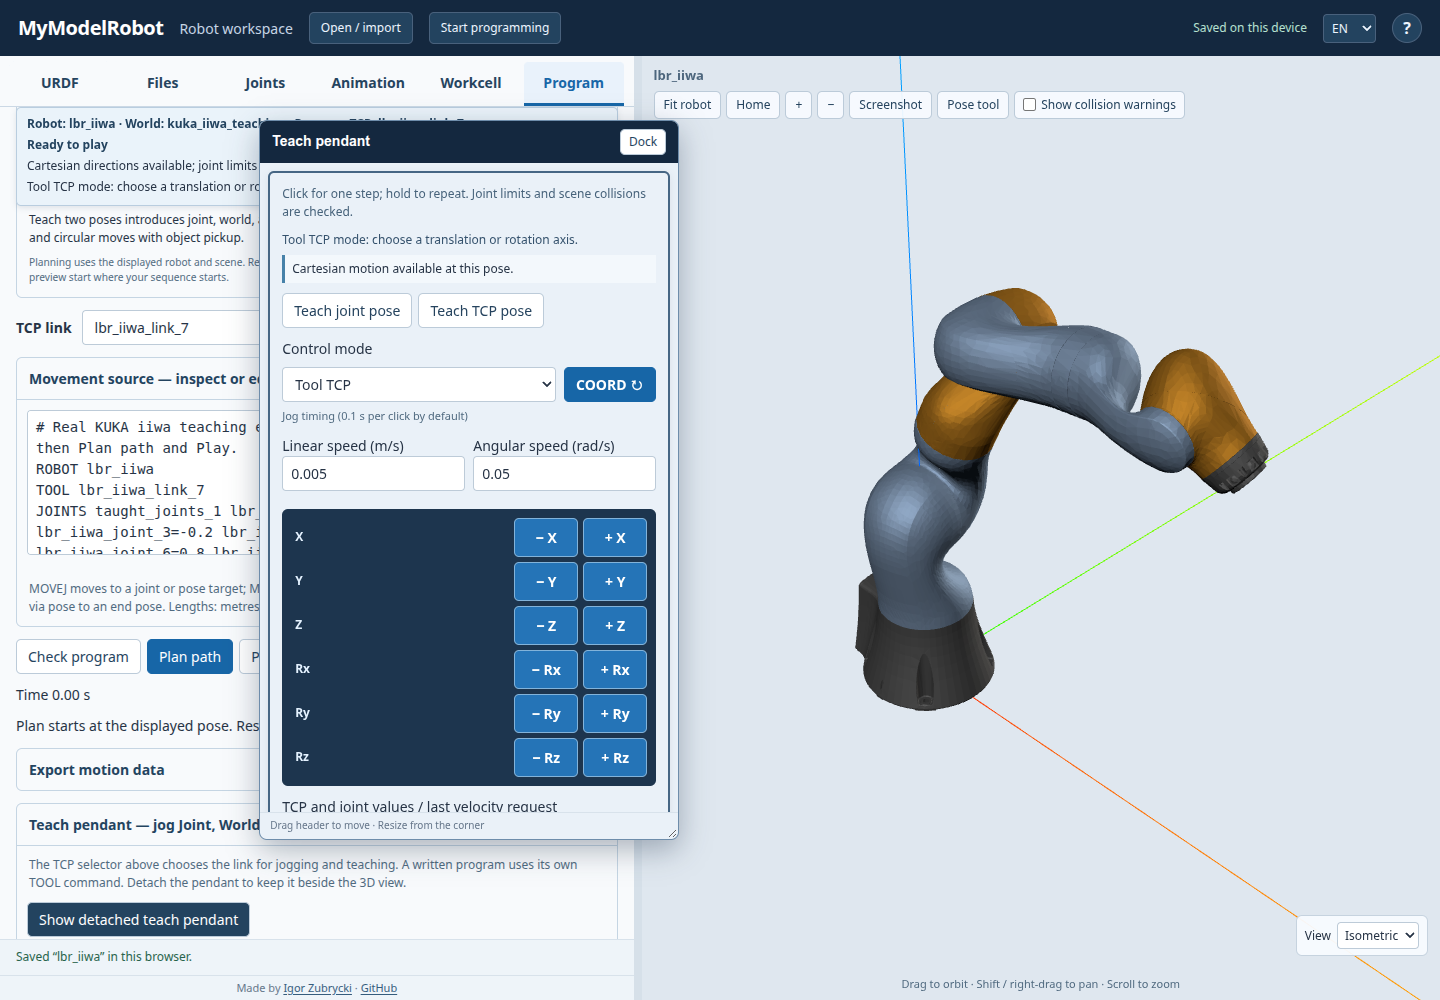
\includegraphics[width=.47\linewidth,height=52mm,keepaspectratio,trim=700 140 20 140,clip]{assets/kuka.png}\hfill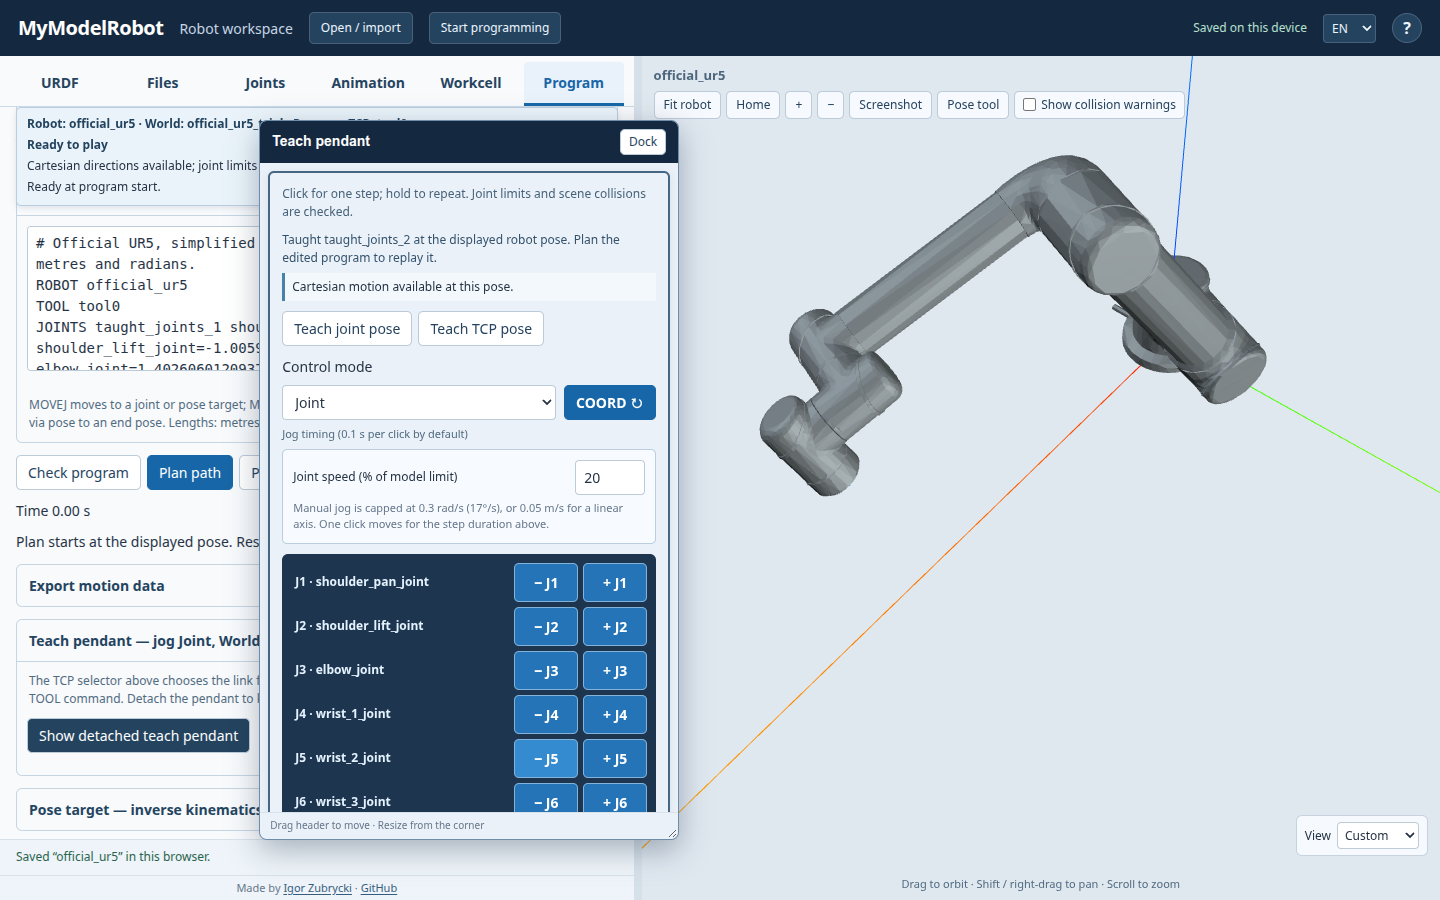
\includegraphics[width=.47\linewidth,height=52mm,keepaspectratio,trim=700 110 20 100,clip]{assets/ur5.png}\end{center}
\textit{Modele sprawdzone w przeglądarce. Dla zgodności z obecnym importerem użyto siatek STL także do prezentacji wyglądu. Zachowano łańcuchy kinematyczne i geometrie kolizyjne; nie są to skalibrowane modele konkretnego egzemplarza sprzętu.}
\textbf{Zaliczenie:} własny ZIP poprawnie otwarty ponownie; w rozszerzeniu także ruch na drugim robocie.

\page{Ściąga: program, stan i oddanie ćwiczenia}{Do użycia podczas samodzielnej pracy}
\begin{tabularx}{\linewidth}{@{}p{68mm}X@{}}\toprule
\textbf{Zapis / przycisk}&\textbf{Znaczenie}\\\midrule
\cmd{ROBOT nazwa}&Wybór robota dla programu; nazwa musi pasować do modelu.\\
\cmd{TOOL link}&Wybór istniejącego linku TCP; to nazwa układu, nie sześć liczb offsetu.\\
\cmd{POSE p world x y z Q qx qy qz qw}&Pełna pozycja i orientacja celu w świecie; kolejność kwaternionu \(xyzw\).\\
\cmd{POSE p world x y z AA ax ay az angle}&Ta sama idea orientacji jako oś i kąt w radianach; nie kąty Eulera.\\
\cmd{JOINTS p joint=value ...}&Nazwany cel złączowy; metry dla złączy liniowych, radiany dla obrotowych.\\
\cmd{MOVEJ p} / \cmd{MOVEL p}&Ruch do celu / odcinek TCP. MOVEL wymaga celu POSE.\\
\cmd{MOVEC via end}&Łuk: start bieżący, pozycja pośrednia i koniec; dwa nazwane cele POSE.\\
\cmd{PAUSE seconds}&Oczekiwanie zapisane w programie.\\
\cmd{GRAB object} / \cmd{RELEASE object}&Przyłączenie obiektu do TCP / odłączenie z zachowaniem pozycji w świecie.\\
\cmd{ZONE 0}&Dokładne zatrzymania na granicach ruchów. Dodatnia wartość w metrach żąda lokalnego wygładzenia obsługiwanych przejść; nie utożsamiaj jej z dokładnością kątową.\\
\ui{Check program} / \ui{Plan path}&Sprawdzenie składni / obliczenie wykonalnego ruchu dla bieżącego stanu.\\
\ui{Play / Pause / Reset / Step}&Odtwarzanie / pauza / powrót do początku planu / następna próbka czasu.\\\bottomrule
\end{tabularx}
\begin{remember}\textbf{Gdy coś nie działa:} odczytaj aktywnego robota i TCP, stan planu, ostrzeżenie o postawie, a dopiero potem ostatni komunikat błędu. Przy braku planu nie oczekuj działania Play. Nie wyłączaj ostrzeżeń w nadziei na naprawienie toru.\end{remember}
\textbf{Co oddać?} Jeden ZIP własnego programu dwóch punktów, jeden zrzut toru odcinków i łuku, krótka tabela World/Tool oraz opis jednej nieudanej próby i jej poprawienia. Dołącz nazwy robota/TCP, jednostki, sposób przywrócenia początku i odpowiedzi na pytania z ćwiczeń.

\begin{tabularx}{\linewidth}{@{}Xr@{}}\toprule
\textbf{Proponowane kryteria oceny}&\textbf{Punkty}\\\midrule
Rozróżnienie Joint/World/Tool na podstawie pomiarów&4\\
Uczenie A/B, jawny początek, poprawny plan i odtwarzanie&5\\
Interpretacja odcinka, łuku i punktu pośredniego&4\\
Diagnoza ograniczenia/kolizji oraz poprawne przywrócenie stanu&4\\
Kompletny i odtwarzalny ZIP, jasne krótkie wnioski&3\\\midrule
Razem&20\\\bottomrule
\end{tabularx}
\textbf{Dla prowadzącego.} Sprawdź świeżą lekcję i przykład pick-and-place przed zajęciami. Do pracy podstawowej wystarczają ćwiczenia 1--6. Rozszerzeniem mogą być własny tor, drugi robot, analiza ZONE albo demonstracja procesu \cmd{WELD ON/OFF} w przykładzie spawania; jest to adnotacja ścieżki, bez modelu cieplnego i wytrzymałości spoiny.

{\footnotesize\textbf{Materiały i pochodzenie.} Instrukcja opisuje lokalną wersję MyModelRobot z dnia 14.11.2026 i sprawdzone przykłady aplikacji. Inspiracja metodyczna: Politechnika Łódzka, \textit{Robotyka, ćwiczenie C: Symulacja pracy robotów w środowisku EASY-ROB}, udostępniony materiał laboratoryjny, \href{https://automatyka.p.lodz.pl/sites/i21/files/2026-02/stanowisko_c_-_easy-_rob.pdf}{adres źródła}. Ćwiczenia i ilustracje dotyczą MyModelRobot; znajomość tego materiału nie jest potrzebna. Pochodzenie modeli i licencje znajdują się w \cmd{README.md} pakietu.}
\end{document}
